\documentclass[conference]{IEEEtran}
\IEEEoverridecommandlockouts
\usepackage{cite}
\usepackage{amsmath,amssymb}
\usepackage{graphicx}
\usepackage{booktabs}
\usepackage{textcomp}
\usepackage{xcolor}
\usepackage{fontspec}
\setmainfont{texgyretermes}[Extension=.otf,UprightFont=*-regular,BoldFont=*-bold,ItalicFont=*-italic,BoldItalicFont=*-bolditalic]
\setsansfont{texgyreheros}[Extension=.otf,UprightFont=*-regular,BoldFont=*-bold,ItalicFont=*-italic,BoldItalicFont=*-bolditalic]
\setmonofont{texgyrecursor}[Extension=.otf,UprightFont=*-regular,BoldFont=*-bold,ItalicFont=*-italic,BoldItalicFont=*-bolditalic]

\begin{document}

\title{How Do Linear, Kernel and Convolutional Classifiers Fail Under Image Degradation? A Controlled Comparison on Fashion-MNIST and ciFAIR-10}

\author{\IEEEauthorblockN{Shreya Gunjkar, Aarushi Nishant Singh, Kashish Bharti, and Neel Patel}
\IEEEauthorblockA{\textit{Department of Computer Engineering and Technology, School of Computer Science and Engineering}\\
\textit{Dr Vishwanath Karad MIT World Peace University}\\
Pune, India\\
shreya.gunjkar@mitwpu.edu.in, aarushi.singh@mitwpu.edu.in, kashish.bharti@mitwpu.edu.in, neel.patel@mitwpu.edu.in}}

\maketitle

\begin{abstract}
Classifiers are normally evaluated on clean test images, yet they are deployed on images affected by noise, blur, poor contrast or exposure shifts.
We compare three pattern-recognition approaches: linear discriminant analysis on pixels (LDA), an RBF support vector machine on
histogram-of-oriented-gradients features (SVM+HOG), and a small convolutional neural network (CNN). Every model is trained and tuned on clean images only,
frozen, and then scored on test images degraded by Gaussian noise, Gaussian blur, contrast reduction and brightness increase at five audited severities.
Two near-duplicate-filtered datasets are used (Fashion-MNIST and ciFAIR-10), all models receive bit-identical degraded images, and differences are assessed with
paired bootstrap intervals and Holm-corrected exact McNemar tests. The CNN is the most accurate model on clean data (0.928 and about 0.80), but this ranking
does not persist under degradation: on Fashion-MNIST it is significantly less accurate than SVM+HOG in 16 of 21 conditions. On Fashion-MNIST, HOG-based models are almost unaffected by
contrast and brightness changes but sensitive to noise, LDA is the most tolerant of noise and blur, and failing models collapse onto a few predicted classes.
The accuracy of the CNN under a single degradation varies by up to 0.12 across training seeds, although its clean accuracy varies by only 0.001.
\end{abstract}

\begin{IEEEkeywords}
robustness, image degradation, pattern recognition, histogram of oriented gradients, convolutional neural network, linear discriminant analysis
\end{IEEEkeywords}

\section{Introduction}
Image classifiers are usually developed on clean benchmark images, whereas images met in practice are degraded by sensor noise, defocus, poor illumination or
low contrast. A model that scores well on clean data can lose much of its accuracy when the input quality changes, and different families of classifiers
may fail in different ways. Knowing how each family degrades, and under which degradation, matters when a method must be chosen for a setting in which the
quality of the input is not controlled.

This paper reports a controlled comparison; it proposes no new algorithm. We ask three questions. \emph{RQ1:} how does the accuracy of a linear statistical
classifier, a hand-crafted-feature kernel classifier and a convolutional network change as test images are degraded by four types of degradation at five
severities? \emph{RQ2:} does the ranking of the models by clean accuracy persist under degradation? \emph{RQ3:} how do the models fail, that is, are errors spread over
the classes or concentrated on a few?

The contributions are methodological and empirical. (i) Near-duplicate-filtered versions of two benchmarks. (ii) A degradation ladder that is audited and frozen before
any model is evaluated. (iii) A freeze-then-evaluate protocol: models are trained and tuned on clean data, hashed, and scored on degraded test images that are
bit-identical for every model. (iv) Paired statistical comparisons with bootstrap intervals and multiple-comparison correction. (v) An account of how the three
model families fail, including the effect of the CNN training seed.

\section{Related Work}
\textbf{Corruption benchmarks and degradation studies.} The usual way to measure robustness is to apply graded, model-agnostic corruptions to a test set and record the
loss in accuracy; ImageNet-C and its companions made this protocol standard \cite{hendrycks2019}, and MNIST-C applied the idea to a small grayscale dataset \cite{mu2019}.
Earlier studies had already shown that deep networks trained on clean images lose accuracy under blur and noise \cite{dodge2016,vasiljevic2016}, and the
relation between such distortions and human recognition was examined as well \cite{dodge2017}. A review of non-adversarial robustness in computer vision
frames the problem in causal terms and stresses how much less attention it has received than adversarial robustness \cite{drenkow2022}.

\textbf{Recent benchmarks and surveys.} Recent work refines how corruptions are generated and judged. A WACV 2024 framework produces benchmarks with adjustable distortion
levels \cite{sarkar2024}; another study measures robustness over a continuous range of corruption strength against the performance of human participants and reports a larger gap
between networks and humans than previously known \cite{shen2024}; a large benchmark compares 55 ImageNet models and finds a trade-off between adversarial and natural
robustness within an architecture \cite{liu2023}; and a survey of corruption robustness organises remedies into augmentation, learning strategies and network components, noting that
robustness does not reliably grow with model or data size \cite{wang2024}. These works concern large natural-image datasets and deep networks.

\textbf{Remedies.} Several recent IEEE-published papers start from a trained network: one consolidates convolutional filters through sleep-like replay to make them more robust
\cite{delanois2023}, one selects normalisation statistics according to the detected corruption \cite{camuffo2024}, and one examines how post-hoc pruning affects calibration and corruption robustness \cite{mitra2024}. Another line adds noisy images to the training
set and reports better accuracy on corrupted test images with little change on clean data \cite{ramirez2026}. We do not study remedies; we study how un-remediated models fail.

\textbf{Hand-crafted versus learned features.} The HOG descriptor, which normalises gradient histograms over overlapping blocks, was introduced for human detection \cite{dalal2005}, and gradient-trained
convolutional networks for recognition earlier \cite{lecun1998}. Among the recent studies we found, one combines HOG with deep features under varying noise and reports that the gain from adding HOG is smaller
in noisy conditions \cite{ezuma2026}. We did not find a controlled comparison of a linear classifier, a HOG-feature kernel classifier and a CNN under a frozen degradation ladder with paired tests.

\textbf{Evaluation hygiene.} Near-duplicates between training and test images inflate scores; they are documented for CIFAR-10 \cite{barz2020} and for Fashion-MNIST \cite{geier2019}. Paired tests on the same
test images \cite{dietterich1998} with correction for multiple comparisons \cite{holm1979} are standard in classifier comparison but are seldom reported in corruption-robustness papers.

\section{Methodology}
\begin{figure*}[t]
\centering
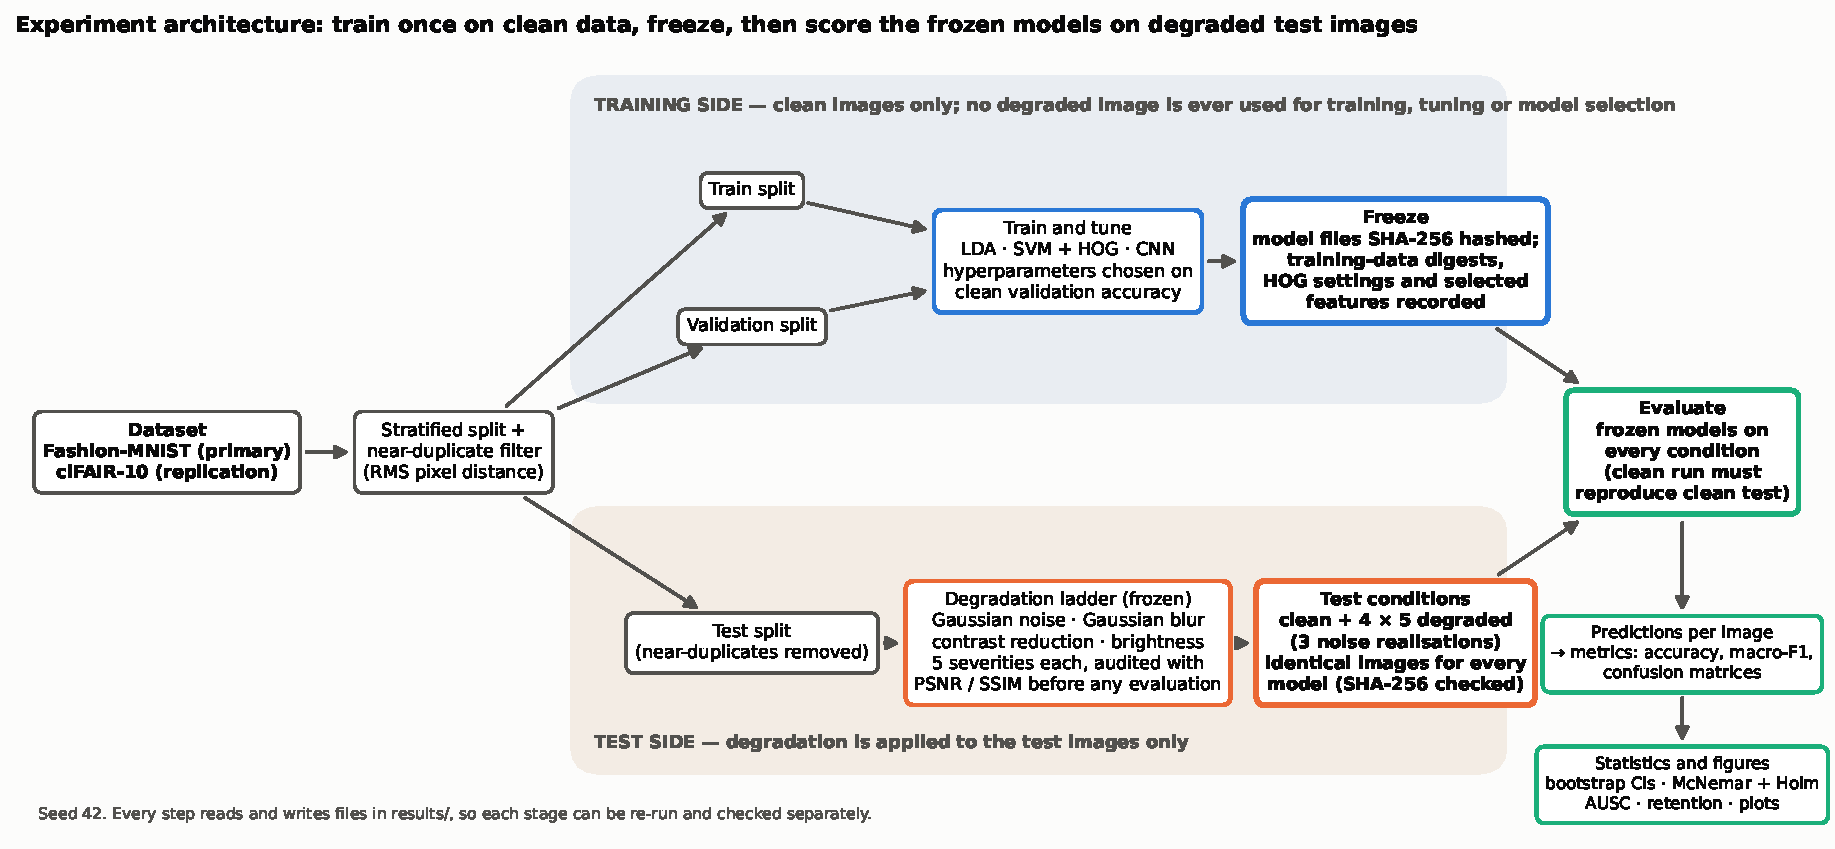
\includegraphics[width=0.92\textwidth]{figs/architecture_system_paper.pdf}
\caption{Experiment architecture. Every model is trained and tuned on clean images only, frozen (hashed), and then scored on test images degraded by a frozen ladder;
the degraded images are identical for every model.}
\label{fig:arch}
\end{figure*}

\subsection{Data and leakage control}
Fashion-MNIST (28$\times$28 grayscale, ten clothing classes) \cite{xiao2017} is the primary dataset and ciFAIR-10 (32$\times$32 RGB, ten classes) the replication dataset;
ciFAIR-10 is CIFAR-10 with the duplicated test images replaced \cite{barz2020}. The official training set is split with a stratified split (seed 42) into training and validation parts.
Near-duplicates are removed using the RMS pixel distance on the $[0,1]$ scale: validation images are compared with the retained training images and test images with the whole
official training set, with thresholds 0.04 (Fashion-MNIST) and 0.08 (ciFAIR-10). The filter removed 14 validation and 18 test images from Fashion-MNIST and 72 and 99 from
ciFAIR-10, leaving 50\,000/9\,986/9\,982 and 45\,000/4\,928/9\,901 training/validation/test images. The thresholds were chosen by inspecting ranked image pairs before any
model existed, so the test set was inspected while the benchmark was built; on CIFAR-style images a pixel threshold cannot separate duplicates from look-alikes, and the
resulting sets are therefore called distance-filtered benchmarks.

\subsection{Degradations}
Four degradations are applied to the test images only, each at five severities. Gaussian noise adds $\sigma z$ with $z\sim\mathcal N(0,1)$ independently per pixel and channel,
$\sigma\in\{0.05,0.10,0.20,0.35,0.50\}$. Gaussian blur uses a separable kernel with mirrored borders, $\sigma\in\{0.5,1,1.5,2,3\}$ pixels. Contrast reduction maps $x$ to $m+\alpha(x-m)$ with $m$ the image mean,
$\alpha\in\{0.75,0.50,0.30,0.15,0.05\}$. Brightness increase adds $\beta\in\{0.1,0.2,0.3,0.4,0.5\}$. Results are clipped to $[0,1]$ and stored as 8-bit integers (Fig.~\ref{fig:grid}).
Noise is generated per image from the seed, the realisation index, the data split and the image identifier, so it does not depend on batch size or order; three independent noise realisations are evaluated.
The severity values were audited on 1\,000 clean training images per dataset with PSNR and SSIM against three criteria declared in advance (monotone decrease with severity,
at least 99\% of images altered at severity 1, at most 1\% constant images at severity 5); all passed, and the ladder was then frozen. PSNR and SSIM measure similarity, not recognition difficulty,
so equal severity numbers do not mean equal difficulty across families.

\begin{figure}[t]
\centering
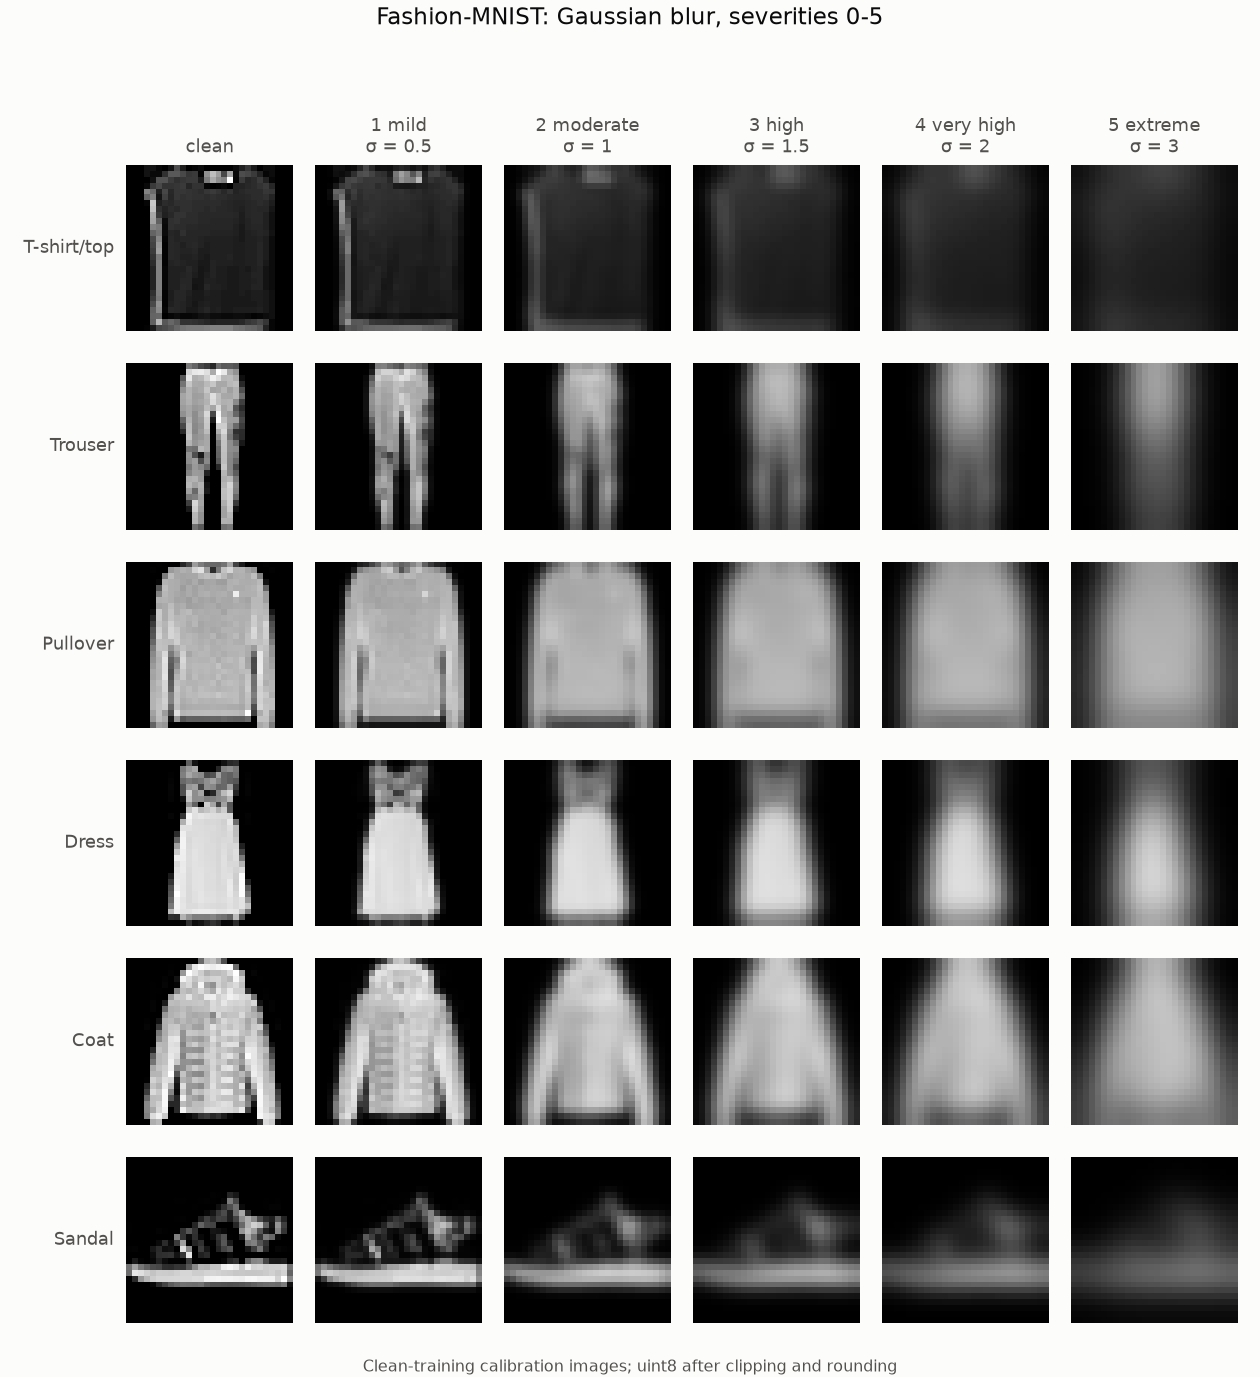
\includegraphics[width=0.98\columnwidth]{figs/degradation_grid_fashion_mnist_gaussian_blur.png}
\caption{Gaussian blur on Fashion-MNIST: one clean training image per class (rows) followed by severities 1--5 (columns).}
\label{fig:grid}
\end{figure}

\subsection{Models}
\textbf{LDA.} One scalar mean and one scalar standard deviation, computed from the clean training images and then frozen, normalise the pixels, which are flattened and
classified by shrinkage LDA. \textbf{SVM+HOG.} HOG features are computed from the unit-scale image after degradation (9 orientations, 4$\times$4-pixel cells, 2$\times$2-cell blocks, L2-Hys
block normalisation; 1\,296 features for 28$\times$28 and 1\,764 for 32$\times$32 images, fixed in advance and not tuned) and classified by an RBF-kernel SVM. HOG and classifier form one model.
\textbf{CNN.} Five 3$\times$3 convolution layers (32, 32, 64, 64 and 128 channels) with batch normalisation and ReLU, two max-pooling and two dropout (0.25) stages, global average pooling and a
linear layer (about 140\,000 parameters); Adam with a one-cycle schedule, batch size 128, 10 epochs, no data augmentation, the epoch with the best clean validation accuracy kept, three training seeds.
\textbf{Feature-selection variants.} Because the course requires a feature-selection algorithm, LDA and SVM+HOG were also trained with an ANOVA F-test filter (\texttt{SelectKBest}) that keeps the top
10--75\% of the pixels or HOG features, ranked on the clean training split and frozen with the model \cite{guyon2003}; they are reported briefly in Section~\ref{sec:fs}. The CNN learns its own features.

\subsection{Freeze-then-evaluate protocol}
All models are trained and tuned on clean data only. Each model file is hashed (SHA-256) together with the digests of its training and validation arrays and its HOG and selection settings, and the
evaluation code refuses a model whose record does not match. The degraded test images are generated once; their digests are verified to be identical for every model, and the clean condition must reproduce the
clean-test predictions exactly. No degraded image is used for training, tuning, epoch selection or model selection.

\section{Experimental Setup}
\textbf{Tuning.} Hyperparameters are chosen by clean validation accuracy. LDA: shrinkage in $\{0.001,0.01,0.05,0.1,0.3,\text{auto}\}$. SVM+HOG: $C\in\{1,10\}$ and an RBF width multiplier in $\{0.5,1,2\}$, tuned on a
stratified 10\,000-image training subset and then refitted on the whole training set. CNN: learning rate $\{0.001,0.003\}\times$ weight decay $\{0,0.0005\}$, each trained for 10 epochs; the best configuration was
retrained with two further seeds. Several selected values lie at the edge of their grids (SVM $C$ and width, the CNN learning rate and weight decay), so the optima may lie outside the grids.

\textbf{Evaluation.} Each model is scored on the clean test set and on 20 degraded conditions (4 families $\times$ 5 severities), with three noise realisations, i.e.\ 31 runs per model and dataset. Metrics are accuracy,
macro-averaged precision, recall and F1, and confusion matrices.

\textbf{Statistics.} (i) Ninety-five-percent percentile bootstrap intervals over test images (2\,000 resamples) with the same resampled images for every model, so that differences are paired; they describe test-set sampling
uncertainty only, and CNN seed variance is reported separately as the range over three seeds. (ii) Exact two-sided McNemar tests on the discordant test images for each pair of models in every condition, Holm-corrected over
all tests of a dataset; for pairs involving the CNN each of the three seeds is tested, and a result counts only if all three agree. For noise conditions the test uses noise realisation~0, whereas reported accuracies average the three realisations;
averaging changes a pairwise difference by at most 0.006. (iii) The area under the severity curve (AUSC), the mean accuracy over severity 0--5.

\textbf{Implementation.} Python 3.12, NumPy 2.5, scikit-learn 1.9, scikit-image 0.26 and PyTorch 2.15 on an Apple M5 CPU; seed 42 throughout (CNN seeds 42--44). Code, frozen-model records, predictions and tables are in the project repository.

\section{Results}
\subsection{Clean performance}
\begin{table}[t]
\caption{Clean test accuracy and macro-F1 (CNN: mean over three seeds, range in parentheses).}
\label{tab:clean}
\centering\small
\resizebox{\columnwidth}{!}{\begin{tabular}{llcc}
\toprule
Dataset & Model & Accuracy & Macro-F1 \\
\midrule
Fashion-MNIST & LDA & 0.817 & 0.817 \\
 & SVM+HOG & 0.911 & 0.911 \\
 & CNN & 0.928 (0.927--0.928) & 0.928 \\
\midrule
ciFAIR-10 & LDA & 0.405 & 0.403 \\
 & SVM+HOG & 0.625 & 0.625 \\
 & CNN & 0.802 (0.798--0.806) & 0.800 \\
\bottomrule
\end{tabular}
}
\end{table}
On clean data the ranking is CNN $>$ SVM+HOG $>$ LDA on both datasets (Table~\ref{tab:clean}). The CNN's lead over SVM+HOG is 0.017 on Fashion-MNIST and 0.17--0.18 on ciFAIR-10, and the SVM adds
0.095 and 0.22 over LDA. Test accuracy is 0.4--2.0 points below validation accuracy for every model, the usual direction for scores that were used to choose hyperparameters.

\subsection{Accuracy under degradation}
\begin{figure*}[t]
\centering
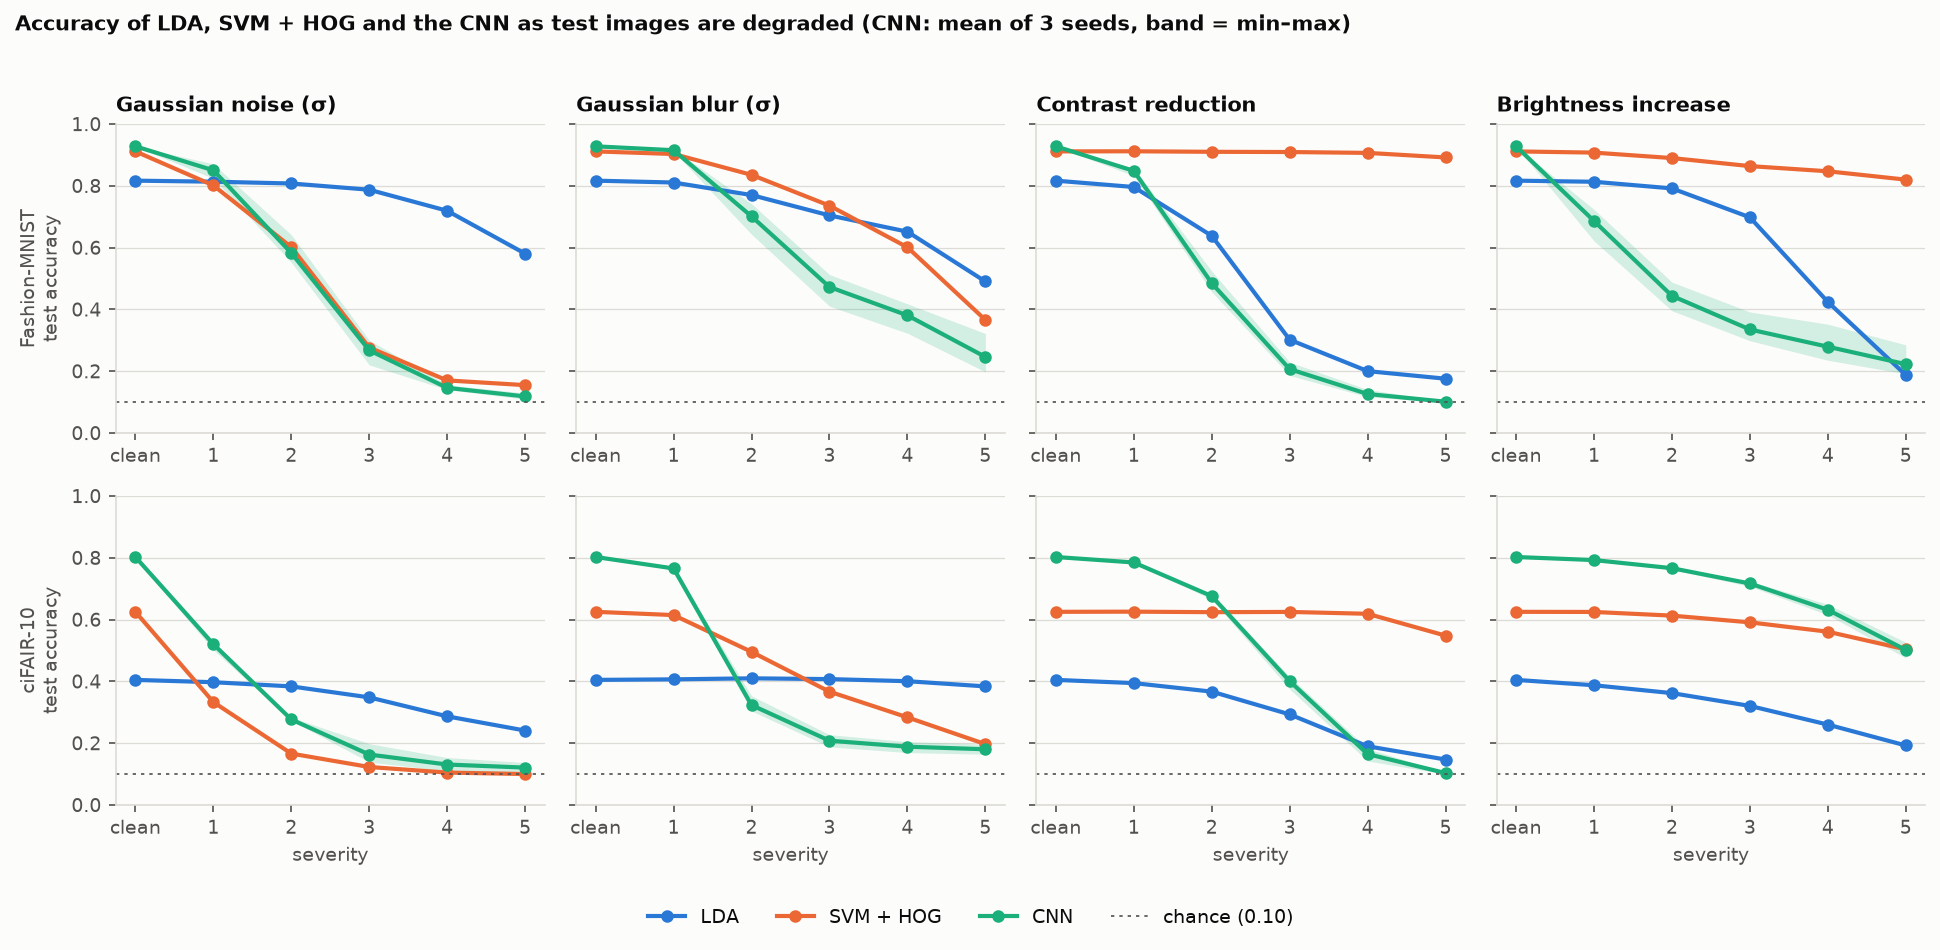
\includegraphics[width=\textwidth]{figs/main_robustness_curves.png}
\caption{Test accuracy of the three models as the degradation severity increases (CNN: mean of three seeds, shaded band = seed range; dotted line = chance).}
\label{fig:curves}
\end{figure*}
Fig.~\ref{fig:curves} shows accuracy against severity. The clean ranking does not persist. On Fashion-MNIST at severity 5 the best model is LDA under noise (0.580) and blur (0.490) and SVM+HOG under
contrast (0.892) and brightness (0.820), while the CNN is lowest of the three under noise (0.118), blur (0.246) and contrast (0.101); under brightness it already falls from 0.928 to 0.686 at severity 1
(seed range 0.622--0.723). On ciFAIR-10 the CNN is the best model at severity 1 under all four degradations, but by severity 5 LDA is best under noise (0.241) and blur (0.384), SVM+HOG under contrast (0.548), and
the CNN and SVM+HOG are level under brightness (0.501 and 0.503).

\begin{table*}[t]
\caption{Area under the severity curve (mean accuracy over severity 0--5); best of the three models in bold. The 95\% bootstrap half-width is at most 0.009.}
\label{tab:ausc}
\centering\small
\begin{tabular}{lcccccc}
\toprule
 & \multicolumn{3}{c}{Fashion-MNIST} & \multicolumn{3}{c}{ciFAIR-10} \\
\cmidrule(lr){2-4}\cmidrule(lr){5-7}
Degradation & LDA & SVM+HOG & CNN & LDA & SVM+HOG & CNN \\
\midrule
Gaussian noise & \textbf{0.765} & 0.476 & 0.474 & \textbf{0.348} & 0.218 & 0.310 \\
Gaussian blur & 0.718 & \textbf{0.743} & 0.611 & 0.404 & \textbf{0.434} & 0.395 \\
Contrast reduction & 0.486 & \textbf{0.908} & 0.436 & 0.304 & \textbf{0.616} & 0.496 \\
Brightness increase & 0.646 & \textbf{0.875} & 0.464 & 0.326 & 0.591 & \textbf{0.712} \\
\bottomrule
\end{tabular}

\end{table*}
The degradation family changes the ranking (Table~\ref{tab:ausc}). HOG-based models are nearly unaffected by contrast reduction on Fashion-MNIST (SVM+HOG 0.911 clean, 0.892 at severity 5) and by moderate brightness shifts, but
sensitive to noise: SVM+HOG falls from 0.625 to 0.333 at severity 1 on ciFAIR-10 and from 0.911 to 0.276 at severity 3 on Fashion-MNIST. Pixel-based LDA is the most tolerant of noise (0.817 to 0.580 at severity 5 on
Fashion-MNIST) and, on ciFAIR-10, of blur (0.405 to 0.384), although from a low clean accuracy. On ciFAIR-10 the CNN is clearly best only under brightness. Under noise on Fashion-MNIST the CNN and SVM+HOG are tied (0.474 and 0.476).

\subsection{Statistical comparison}
\begin{table}[t]
\caption{Number of the 21 conditions (clean and 20 degraded) in which the first or second model is significantly more accurate (exact McNemar test, Holm-corrected, $p<0.05$), not significant (n.s.), or, for the CNN, significant for only some of the three seeds.}
\label{tab:pairs}
\centering\footnotesize
\resizebox{\columnwidth}{!}{\begin{tabular}{llcccc}
\toprule
Dataset & Pair (first vs second) & First & Second & n.s. & Seeds \\
\midrule
Fashion-MNIST & SVM+HOG vs LDA & 14 & 6 & 1 & -- \\
 & CNN vs LDA & 3 & 16 & 0 & 2 \\
 & CNN vs SVM+HOG & 2 & 16 & 0 & 3 \\
\midrule
ciFAIR-10 & SVM+HOG vs LDA & 13 & 8 & 0 & -- \\
 & CNN vs LDA & 11 & 9 & 0 & 1 \\
 & CNN vs SVM+HOG & 11 & 6 & 0 & 4 \\
\bottomrule
\end{tabular}
}
\end{table}
The 95\% bootstrap interval of an accuracy has a half-width of 0.008 on average (0.010 at most), so most differences between models are far larger than test-set sampling noise, and nearly every comparison is significant (Table~\ref{tab:pairs}).
On Fashion-MNIST the CNN is significantly less accurate than SVM+HOG in 16 of 21 conditions and than LDA in 16 (more accurate in 2 and 3; the seeds disagree in 3 and 2). On ciFAIR-10 the CNN is more accurate than SVM+HOG in 11
conditions and less accurate in 6, and in 4 the outcome depends on the seed. The training seed matters far more for the CNN than the noise draw does: across three seeds its accuracy under one degraded condition differs by up to 0.124
(Fashion-MNIST) and 0.059 (ciFAIR-10), whereas re-drawing the noise changes any model's accuracy by at most 0.012.

\subsection{How the models fail}
\begin{figure*}[t]
\centering
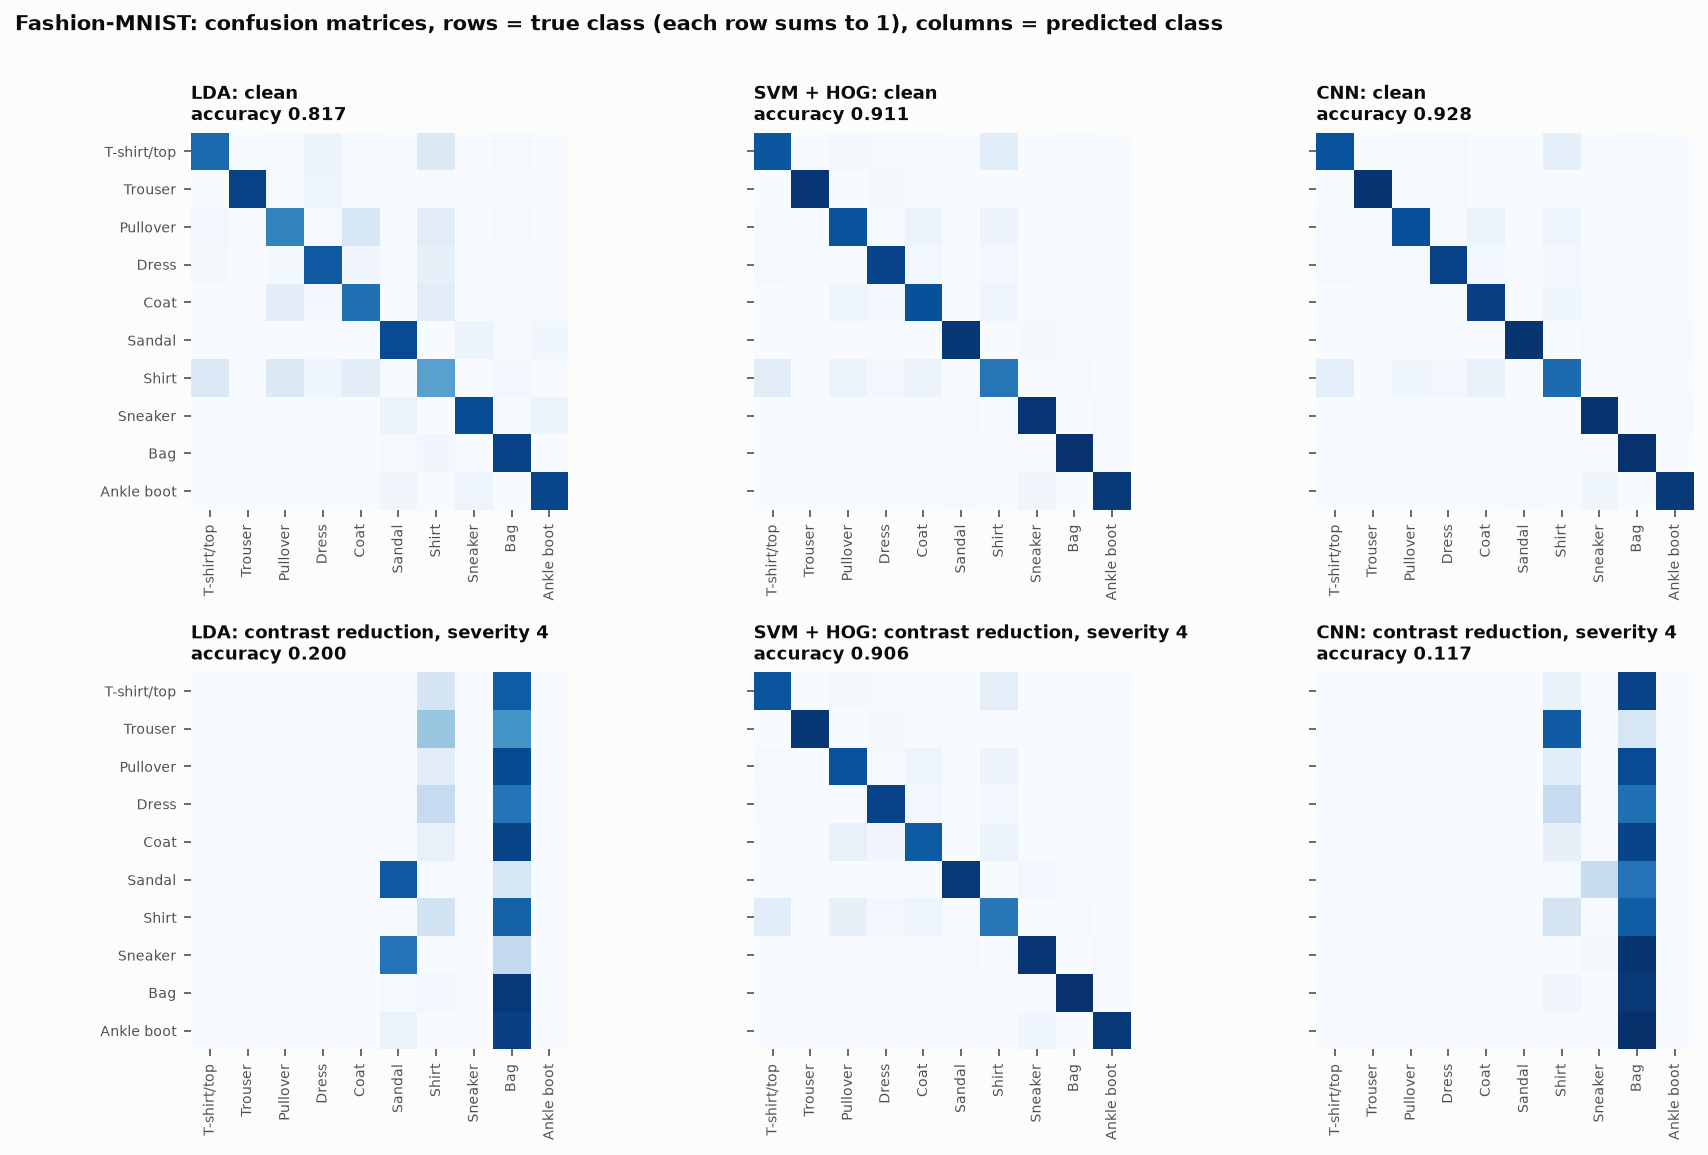
\includegraphics[width=0.62\textwidth]{figs/main_confusion_fashion_mnist.png}
\caption{Row-normalised confusion matrices on Fashion-MNIST for clean images (top) and contrast reduction at severity 4 (bottom). Rows are true classes, columns predicted classes.}
\label{fig:conf}
\end{figure*}
On clean data every model spreads its predictions over the classes: the most-predicted class receives 0.10--0.12 of them. At severity 5 the share of predictions falling in the single most-predicted class (mean over the four
degradations) is 0.78 for the CNN on Fashion-MNIST, against 0.56 for LDA and 0.35 for SVM+HOG, and 0.59 on ciFAIR-10, against 0.40--0.42. Failing models therefore label most images with one or two classes
(Fig.~\ref{fig:conf}). Several conditions end near chance (0.10), where models can no longer be told apart.

\subsection{Feature-selection variants}\label{sec:fs}
Clean validation accuracy rose with the fraction of features kept and the largest fraction offered (75\%) was always selected, so selection gave no consistent significant gain in clean accuracy. Its effect on robustness depended on the model and
dataset: LDA with selection was much more accurate than LDA on Fashion-MNIST under severe brightness increase ($+0.245$, 95\% interval $[+0.237,+0.254]$) but mostly slightly less accurate on ciFAIR-10, except under noise ($+0.054$ at severity 5);
SVM+HOG with selection differed significantly from SVM+HOG in 6 of 21 conditions on Fashion-MNIST (changes of at most 0.03) and 1 of 21 on ciFAIR-10. A non-significant difference does not show that two models are equivalent.

\section{Discussion}
\textbf{Observations.} Clean accuracy is a poor guide to robustness here. The CNN, best on clean data, is the weakest of the three under several degradations on Fashion-MNIST, while SVM+HOG is the most stable under contrast and
brightness changes and LDA under noise and blur. On ciFAIR-10 the orderings change with the degradation and the models are closer, so the Fashion-MNIST ordering should not be generalised. Failing models collapse onto one or two classes, and
the behaviour of the CNN under degradation depends noticeably on the training seed although its clean accuracy does not.

\textbf{Possible explanations (not tested here).} The insensitivity of the HOG-based models to contrast reduction is consistent with block normalisation removing the scale of local gradients, and their tolerance of additive brightness with an
offset leaving gradients unchanged except where pixels clip. Their sensitivity to noise is consistent with gradient computation amplifying independent pixel noise, whereas a linear classifier on raw pixels averages the noise over many pixels.
The loss of the CNN under brightness on Fashion-MNIST is consistent with a network trained without augmentation on an exactly black background, whose stored batch-normalisation statistics no longer match shifted activations. The collapse of failing
models onto a few classes is consistent with degraded inputs moving every sample into a region of feature space that the model assigns to one class. None of these mechanisms was tested, for example by examining activations or removing components.

\textbf{Practical implication.} If the kind of degradation in use is unknown, a model should not be chosen by clean accuracy alone; on Fashion-MNIST, HOG features gave the most stable accuracy under contrast and brightness changes, at the price of sensitivity to noise.

\section{Limitations}
The degradations are synthetic and simple: noise is independent across pixels and channels, blur is isotropic, contrast uses one mean per image, brightness is only positive, and 8-bit storage quantises the strongest contrast reduction.
Severity levels are not equally hard across families. The duplicate thresholds were chosen by looking at test/training pairs. Tuning grids are small, several selected values lie at their edges, the SVM was tuned on a subset, the HOG geometry is fixed,
and the CNN was still improving after 10 epochs. The CNN has only three seeds, the deterministic models were fitted once, and the bootstrap and McNemar analyses treat images as independent and cover test-set sampling only. Results are for one
test set per dataset, two small image datasets and four synthetic degradations; they do not establish that the same ordering holds on other data or on real degraded images.

\section{Conclusion}
Under a controlled protocol in which every model is trained and tuned on clean data only and scored on bit-identical degraded test images, the clean-accuracy ranking CNN $>$ SVM+HOG $>$ LDA did not persist under degradation. On Fashion-MNIST, HOG-based models were the most stable under
contrast reduction and additive brightness (under contrast also on ciFAIR-10) but the most sensitive to Gaussian noise; pixel-based LDA was the most tolerant of noise and blur, from a low clean accuracy; on Fashion-MNIST the CNN fell furthest under noise, blur and contrast and varied strongly
across training seeds; and failing models collapsed onto a few predicted classes. Feature selection did not change this picture consistently. Future work includes more CNN seeds so that seed variance enters the intervals, tests of the proposed mechanisms,
augmentation or noise-aware training to separate inherent robustness from exposure during training, real degraded data, and additional degradation types.

\bibliographystyle{IEEEtran}
\bibliography{refs}

\end{document}
